\documentclass[10pt]{article}



\usepackage[margin=1in]{geometry}
\usepackage[T1]{fontenc}
\usepackage{mathptmx} % scalable Times text+math (fixes microtype font-expansion on this TeX)
\usepackage{helvet}   % Helvetica for figure sans-serif labels (\sffamily)
\usepackage{microtype}
\usepackage{amsmath,amssymb,amsthm}
\usepackage{mathtools}
\usepackage{booktabs}
\usepackage{array}
\usepackage{graphicx}
\usepackage{xcolor}
\usepackage{tikz}
\usepackage{pgfplots}
\pgfplotsset{compat=1.17}
\usetikzlibrary{arrows.meta,positioning,fit,backgrounds,shapes.geometric,calc,decorations.pathreplacing}
\usepackage{algorithm}
\usepackage{algpseudocode}
\usepackage[numbers,sort&compress]{natbib}
\usepackage{caption}
\usepackage{hyperref}
\hypersetup{colorlinks=true,linkcolor=blue!55!black,citecolor=green!45!black,urlcolor=blue!55!black}
\usepackage[capitalise,noabbrev]{cleveref}
\usepackage{colortbl}
\usepackage{pifont}
\usepackage{makecell}
\usepackage{multirow}

% ---- line-number overlap fix (harmless if lineno absent) ----
\usepackage{setspace}
\makeatletter
\AtBeginDocument{\@ifpackageloaded{lineno}{%
  \setlength{\linenumbersep}{6pt}%
  \renewcommand\linenumberfont{\normalfont\scriptsize\color{gray}}%
  \leftlinenumbers}{}}
\makeatother

% ---- placeholders and run-tags (VISIBLE, never mistaken for data) ----
\newcommand{\PH}[1]{{\color{purple}\small[#1]}}
\newcommand{\RES}{{\color{purple}\small[RESULT]}}
\newcommand{\torun}[1]{\par\noindent\fbox{\parbox{0.97\linewidth}{%
  \small\textcolor{blue!60!black}{\textbf{$\gg\!\gg\!\gg$ TO RUN:}}~#1}}\par\vspace{2pt}}

% ---- theorem environments ----
\newtheorem{theorem}{Theorem}
\newtheorem{proposition}{Proposition}
\newtheorem{corollary}{Corollary}
\newtheorem{definition}{Definition}
\newtheorem{remark}{Remark}
\newtheorem{fact}{Fact}

\newcommand{\E}{\mathbb{E}}
\newcommand{\Var}{\operatorname{Var}}
\newcommand{\R}{\mathsf{R}}
\newcommand{\Gcal}{\mathcal{G}}
\newcommand{\W}{\mathsf{W}}
\newcommand{\design}{\mathsf{d}}
\newcommand{\eqdef}{\vcentcolon=}

\captionsetup{font=small,labelfont=bf}
\setlength{\parskip}{2pt}

% ---- publication figure palette + reusable styles ----
\definecolor{floorcol}{HTML}{2A3D66}   % deep indigo: fundamental sufficiency floor
\definecolor{floorlt}{HTML}{DAE0EF}
\definecolor{gapcol}{HTML}{D98A2B}     % amber: closable expressiveness gap
\definecolor{gaplt}{HTML}{F6E6CC}
\definecolor{okcol}{HTML}{3F7D53}      % green: graph-determined / below tolerance
\definecolor{oklt}{HTML}{DCEADE}
\definecolor{simcol}{HTML}{A23B3B}     % muted red: simulation-required
\definecolor{ink}{HTML}{25303A}        % near-black cool ink
\definecolor{edgegray}{HTML}{8A94A0}
\definecolor{panelbg}{HTML}{F7F8FA}
\tikzset{
  >={Stealth[length=2.4mm,width=1.7mm]},
  fignode/.style={font=\sffamily\small, text=ink},
  figsmall/.style={font=\sffamily\scriptsize, text=ink},
  panel/.style={rounded corners=3pt, draw=edgegray!55, fill=panelbg, line width=0.5pt},
  chip/.style={rounded corners=2.5pt, draw=ink, fill=white, line width=0.7pt,
               font=\sffamily\small, inner sep=4pt, text=ink, align=center},
  gnode/.style={circle, draw=ink, fill=floorlt, line width=0.6pt,
                minimum size=5mm, inner sep=0pt, font=\sffamily\scriptsize},
  lever/.style={line width=1.5pt, -{Stealth[length=2.8mm,width=2.1mm]}},
}
\pgfplotsset{
  every axis/.append style={
    line width=0.7pt,
    tick style={line width=0.6pt, color=edgegray},
    label style={font=\sffamily\small, text=ink},
    tick label style={font=\sffamily\scriptsize, text=ink},
    legend style={font=\sffamily\scriptsize, draw=edgegray!55, fill=white,
                  rounded corners=2pt, text=ink},
    title style={font=\sffamily\small\bfseries, text=ink},
  },
}
\newcommand{\panellab}[1]{{\sffamily\bfseries #1}}

% ---- table styling: glyphs, shades, header cells ----
\definecolor{headbg}{HTML}{ECEFF5}   % neutral header shade
\definecolor{oursbg}{HTML}{FBEBD1}   % amber highlight for our row (positioning, not a result)
\newcommand{\yes}{\textcolor{okcol}{\ding{51}}}
\newcommand{\no}{\textcolor{black!25}{\ding{55}}}
\newcommand{\halfmark}{\textcolor{gapcol}{\large\raisebox{-0.12ex}{$\circ$}}}
\renewcommand{\theadfont}{\sffamily\bfseries\footnotesize}
\renewcommand{\theadalign}{bc}
\renewcommand{\cellalign}{tl}
\arrayrulecolor{black!78}

% ===================================================================
\title{\vspace{-1.2em}\textbf{When Can a Graph Replace a Simulator?\\[2pt]
A Representation-Sufficiency Boundary for\\ GNN-Based Analog Circuit Performance Prediction}}

\author{Anonymous Author(s)\\ \small Submission under double-blind review}
\date{}
% ===================================================================

\begin{document}
\maketitle

\begin{abstract}
Graph neural networks (GNNs) promise to replace slow SPICE simulation for analog performance prediction: a circuit is a graph, and a GNN can in principle read gain, bandwidth, noise figure, or power straight off the diagram. Which of these properties a GNN can predict, and which require simulation, is unresolved. The field pursues this by building ever more expressive encoders (attention over physical flow, higher-order and subgraph GNNs) and richer graph abstractions (net-level, terminal-level) that distinguish circuits standard message passing confuses. Recent state-of-the-art work treats the choice of graph abstraction as a first-order design decision and reports accuracy that varies across metrics, without explaining why the variation persists. We argue this reflects two limits that behave very differently and are routinely conflated. \emph{Encoder expressiveness} governs how well a GNN separates the graphs it is given, and a large literature steadily improves it. \emph{Representation sufficiency} governs whether the chosen graph encoding \emph{contains} the information a property depends on at all; no encoder, at any expressiveness, can recover information the representation has discarded. Applying the classical conditional-variance identity to the representation splits any GNN's squared error into a \emph{representation-sufficiency floor}, which is encoder-independent, and a \emph{closable expressiveness gap}; the floor is the property variance left unexplained within representation-equivalence classes. Our contribution is not that identity but what follows from it here: we identify the message-passing gap in closed form, and we characterize when the floor forces information beyond the netlist. We then turn the graph abstractions the circuit-GNN literature actually debates, from bare topology through net-level and terminal-level graphs with sized devices, into a measuring ladder, and specify a protocol that estimates the per-property floor at each rung on two public benchmarks: FALCON, a dataset of one million Cadence-simulated mm-wave circuits whose labels include noise figure and DC power, and the Open Circuit Benchmark. The protocol is designed to locate, for each property, the minimum representation at which its floor reaches tolerance. The floor analysis is training-free, so an impossibility at a rung cannot be blamed on optimization. A property whose floor vanishes at a coarse rung is graph-determined there, so better architectures suffice; one whose floor persists at the richest practical representation admits no GNN shortcut over simulation. Which properties fall where, and whether any floor persists at the richest rung, are empirical questions our protocol answers rather than assumes. This yields a per-property, evidence-based account of where AI can and cannot substitute for the simulator, and tells practitioners when to invest in architectures versus richer inputs. Quantitative results are pending the experiments specified herein; all reported numbers in this draft are visible placeholders.
\end{abstract}

% ===================================================================
\section{Introduction}
% ===================================================================

A circuit is naturally a graph: components are nodes and wires are edges. Building on this, GNNs have been proposed as fast surrogates that predict analog performance directly from the circuit graph, sidestepping the cost of a full SPICE solve. The Open Circuit Benchmark (OCB) and CktGNN established the setting for operational amplifiers \citep{dong2023cktgnn}; FALCON trains a GNN on one million Cadence-simulated mm-wave circuits spanning twenty topologies and five circuit families, and reports under ten percent relative error in performance prediction \citep{mehradfar2025falcon}. Related work generates topologies \citep{gao2025analoggenie}, predicts missing links at port-level granularity \citep{pan2025gnnaclp}, and a broad survey documents the momentum behind GNNs for electronic design automation \citep{sanchez2023survey}. The animating hope is a boundary: some properties can be read off the graph instantly, and some cannot; knowing which is which tells us where learning replaces simulation.

The field pursues this boundary on two fronts, both aimed at the \emph{model}. The first makes the \emph{encoder} more powerful. Standard message-passing GNNs are bounded by the one-dimensional Weisfeiler--Leman test (1-WL) and cannot distinguish certain non-isomorphic graphs \citep{xu2019gin,morris2019wl,weisfeiler1968reduction}; because some electrically different circuits collapse to the same standard-GNN representation, recent work builds encoders that separate them, most directly flow attention that respects Kirchhoff's current law and distinguishes a circuit from its computation tree \citep{plettenberg2025flow}, alongside higher-order and subgraph GNNs \citep{morris2019wl,bevilacqua2022esan} and positional or random features that break symmetries \citep{sato2021random,loukas2020cannotlearn}. The second makes the \emph{graph abstraction} richer: recent state-of-the-art RF work compares net-level, component-level, and terminal-level circuit graphs and reports that terminal-level detail is essential for some metrics and net-level detail for others \citep{asadi2025rfinformed}. Both fronts share an implicit premise: a property a current model predicts poorly is waiting for a better model, whether a more expressive encoder or a finer representation.

That premise sits awkwardly with the field's own design choices. The RF state of the art models circuits at the device-terminal level precisely to preserve fine-grained connectivity and transistor-level symmetry, and reports an average mean relative error of $3.45\%$ across active RF circuit classes \citep{asadi2025rfinformed}; the choice of representation, more than the choice of encoder, carries that result. FALCON reports under ten percent relative error in performance prediction from a graph derived natively from Cadence netlists \citep{mehradfar2025falcon}, and flow attention improves op-amp prediction by separating circuits that standard message passing merges \citep{plettenberg2025flow}. Each of these studies reports accuracy per metric, and the reported accuracy varies across metrics. We read that spread as the signature of a limit no architecture can move, and argue that naming it changes what to do next.

The two fronts act on two distinct limits that must be separated, because they have opposite remedies (\cref{fig:teaser}). The first is \textbf{encoder expressiveness}: given a fixed graph encoding of a circuit, how well can a GNN separate the encodings it is handed? This is what flow attention, $k$-WL, and subgraph methods improve, and it is genuinely improvable. The second is \textbf{representation sufficiency}: does the graph encoding \emph{contain} the information a property depends on in the first place? Two circuits that are identical as annotated graphs, same topology, same component types, same sized-device values, same terminal assignments, but that differ in a target property, can never be separated by \emph{any} function of that graph, because they are the same input. When a property depends on information the graph abstraction discards, such as bias-dependent small-signal parameters, device-model coefficients beyond the sized values, parasitics, or matching, no encoder at any expressiveness recovers it. No improvement to the architecture can help, because the information is absent from its input. Enriching the graph abstraction, the second front, can raise the ceiling, but only up to the information the richest usable representation still omits, and pushing further means adding back what the simulator computes. The RF SOTA's observation that representation choice, not architecture, governs per-metric accuracy is exactly this second limit surfacing without a name \citep{asadi2025rfinformed}.

The practical stakes are direct. If bandwidth is limited by the sufficiency floor rather than by the encoder, then a paper that improves a GNN's bandwidth prediction with a cleverer attention mechanism may be closing a gap that was already closed, while the residual error it cannot touch is the fundamental one. Distinguishing the two limits tells a practitioner, per property, whether to invest in \emph{better architectures} or in \emph{richer inputs and simulation}. It also converts the informal ``which properties need simulation'' question into a measurable quantity.

\paragraph{Contributions.}
\begin{itemize}\itemsep2pt
\item \textbf{A decomposition that separates the two limits, and an exact formula for the gap.} We split the squared error of \emph{any} predictor that factors through a graph representation $\R$, including every GNN on $\R$, into a \emph{representation-sufficiency floor} $\E[\Var(P\mid \R)]$, which is encoder-independent, and an \emph{expressiveness gap} the encoder class controls (\cref{thm:decomp,cor:indep}). The base decomposition is the classical conditional-variance identity \citep{hastie2009esl,devroye1996probabilistic,cover2006information}, and recent theory shows a sufficiently expressive encoder preserves the representation's information \citep{shen2025graphsufficiency}, so the floor is the operative limit; we claim no novelty there. The new results make the split operational for circuit GNNs: we prove the gap of the dominant message-passing class equals, in the capacity limit, the Bayes-regressor variance across circuits that are distinct yet $1$-WL-indistinguishable, so higher-order and flow encoders reduce a conditional variance across the $1$-WL coarsening and provably never touch the floor (\cref{thm:wlgap,cor:mono}); and at the finest representation the floor equals the property's variance from factors outside the graph-encodable design, which is zero exactly when the property is a deterministic function of that design, characterizing precisely when no GNN can replace simulation (\cref{prop:ladder}).
\item \textbf{A representation ladder as a measuring instrument.} We turn the graph abstractions the circuit-GNN literature actually debates, from bare topology through typed topology, sized-device features, and net-level versus terminal-level ported netlists \citep{dong2023cktgnn,asadi2025rfinformed,plettenberg2025flow} (\cref{tab:ladder}), into a ladder, with estimators for the per-rung sufficiency floor and bootstrap confidence intervals (\cref{sec:estimators}). The headline floor analysis is \emph{training-free}: it is a property of the data and the representation, so an impossibility at a rung cannot be blamed on optimization. The ladder makes the RF SOTA's qualitative ``align the representation with the physics'' guidance \citep{asadi2025rfinformed} into a measured quantity.
\item \textbf{A per-property simulation boundary on two public benchmarks.} We lay out a protocol (positive control first) that estimates, for gain, bandwidth, noise figure, and DC power on FALCON \citep{mehradfar2025falcon} and for gain, bandwidth, phase margin, and figure of merit on OCB \citep{dong2023cktgnn}, whether each property is graph-determined (floor near zero) or graph-underdetermined (floor high even at the richest rung), and pairs each floor with the best achievable GNN error across an expressiveness ladder (\cref{sec:experiments}). Because FALCON labels noise figure and DC power natively, metrics that earlier work could obtain only by re-simulation are measured here from released data. All quantitative claims are placeholders pending these runs.
\end{itemize}

The scope of this draft is limited accordingly. It contributes a framework, an instrument, and a lower bound that holds by construction; the empirical boundary is only as strong as the runs specified here, which must be completed before any numeric claim is made.

% ---------------- TEASER FIGURE ----------------
\begin{figure}[t]
\centering
\resizebox{\linewidth}{!}{%
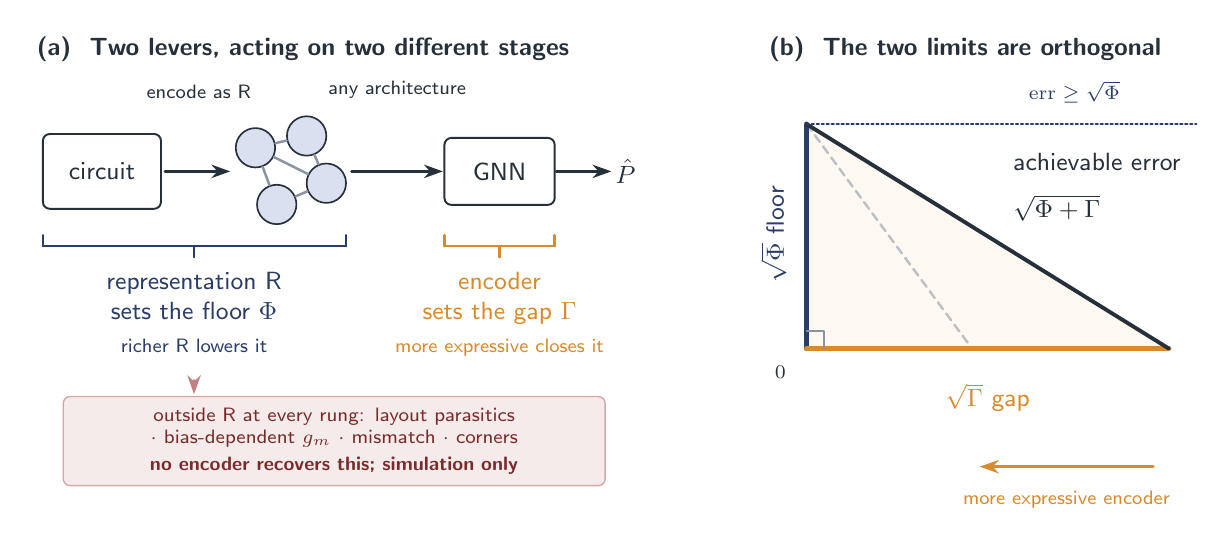
\begin{tikzpicture}[font=\sffamily, line cap=round, line join=round]

% ===================== PANEL (a) =====================
\node[fignode, font=\sffamily\bfseries\small, anchor=west] at (0.00,6.55)
  {(a)\ \ Two levers, acting on two different stages};

% ---- pipeline ----
\node[chip, minimum width=1.5cm, minimum height=0.95cm] (ckt) at (0.95,5.00) {circuit};
\begin{scope}[shift={(3.35,5.00)}]
  \node[gnode] (h1) at (-0.45, 0.30) {};
  \node[gnode] (h2) at ( 0.20, 0.45) {};
  \node[gnode] (h3) at ( 0.45,-0.15) {};
  \node[gnode] (h4) at (-0.18,-0.42) {};
  \draw[edgegray, line width=0.9pt] (h1)--(h2) (h2)--(h3) (h3)--(h4) (h4)--(h1) (h1)--(h3);
\end{scope}
\node[chip, minimum width=1.4cm, minimum height=0.85cm] (gnn) at (6.00,5.00) {GNN};
\node[fignode] (phat) at (7.60,5.00) {$\hat P$};
\draw[->, line width=0.9pt, ink] (1.75,5.00) -- (2.58,5.00);
\draw[->, line width=0.9pt, ink] (4.12,5.00) -- (5.28,5.00);
\draw[->, line width=0.9pt, ink] (6.72,5.00) -- (7.42,5.00);
\node[figsmall, anchor=south] at (2.18,5.80) {encode as $\R$};
\node[figsmall, anchor=south] at (4.70,5.80) {any architecture};

% ---- span brackets tie each lever to the stage it acts on ----
\draw[floorcol, line width=0.9pt] (0.20,4.05) -- (4.05,4.05);
\draw[floorcol, line width=0.9pt] (0.20,4.05) -- (0.20,4.19);
\draw[floorcol, line width=0.9pt] (4.05,4.05) -- (4.05,4.19);
\draw[floorcol, line width=0.9pt] (2.12,4.05) -- (2.12,3.91);
\draw[gapcol, line width=0.9pt] (5.30,4.05) -- (6.70,4.05);
\draw[gapcol, line width=0.9pt] (5.30,4.05) -- (5.30,4.19);
\draw[gapcol, line width=0.9pt] (6.70,4.05) -- (6.70,4.19);
\draw[gapcol, line width=0.9pt] (6.00,4.05) -- (6.00,3.91);

\node[floorcol, font=\sffamily\small, anchor=north, align=center] at (2.12,3.85)
  {representation $\R$\\ sets the floor $\Phi$\\[1pt]{\scriptsize richer $\R$ lowers it}};
\node[gapcol, font=\sffamily\small, anchor=north, align=center] at (6.00,3.85)
  {encoder\\ sets the gap $\Gamma$\\[1pt]{\scriptsize more expressive closes it}};

\draw[->, simcol!65, line width=0.8pt] (2.12,2.35) -- (2.12,2.17);
\node[anchor=north, rounded corners=2.5pt, fill=simcol!10, draw=simcol!45, line width=0.5pt,
      text=simcol!75!black, font=\sffamily\scriptsize, align=center, inner sep=4pt,
      text width=6.6cm] at (3.90,2.15)
  {outside $\R$ at every rung: layout parasitics $\cdot$ bias-dependent $g_m$ $\cdot$
   mismatch $\cdot$ corners\\[2pt]\textbf{no encoder recovers this; simulation only}};

% ===================== PANEL (b) =====================
\node[fignode, font=\sffamily\bfseries\small, anchor=west] at (9.30,6.55)
  {(b)\ \ The two limits are orthogonal};
\begin{scope}[shift={(9.90,2.75)}]
  \coordinate (o)  at (0,0);
  \coordinate (ap) at (0,2.85);
  \coordinate (bp) at (4.60,0);
  \coordinate (bs) at (2.10,0);
  \fill[gapcol!6] (o)--(ap)--(bp)--cycle;
  \draw[ink!30, densely dashed, line width=0.9pt] (ap)--(bs);
  \draw[gapcol!45, line width=1.2pt] (o)--(bs);
  \draw[floorcol, line width=1.9pt] (o)--(ap);
  \draw[gapcol,  line width=1.9pt] (o)--(bp);
  \draw[ink,     line width=1.4pt] (ap)--(bp);
  \draw[edgegray, line width=0.6pt] (0.22,0)--(0.22,0.22)--(0,0.22);
  \draw[floorcol, densely dotted, line width=0.8pt] (ap) -- ++(4.95,0);
  \node[floorcol, font=\sffamily\scriptsize, anchor=south] at (3.40,2.99)
    {$\mathrm{err}\ge\sqrt{\Phi}$};
  \node[floorcol, font=\sffamily\small, rotate=90, anchor=center] at (-0.42,1.45)
    {$\sqrt{\Phi}$ floor};
  \node[ink, font=\sffamily\small, anchor=west, align=left] at (2.50,2.05)
    {achievable error\\[6pt]$\sqrt{\Phi+\Gamma}$};
  % gap label kept well clear of the leg above and of the shrink arrow below
  \node[gapcol, font=\sffamily\small, anchor=north] at (2.30,-0.32) {$\sqrt{\Gamma}$ gap};
  \draw[->, gapcol, line width=1.1pt] (4.40,-1.50) -- (2.20,-1.50);
  \node[gapcol, font=\sffamily\scriptsize, anchor=north] at (3.30,-1.68)
    {more expressive encoder};
  \node[fignode, font=\sffamily\scriptsize, anchor=north east] at (-0.14,-0.10) {$0$};
\end{scope}

\end{tikzpicture}%
}
\caption{\textbf{Two limits, opposite remedies.}
\panellab{(a)}~A GNN sees only the graph representation $\R$, and the two levers act on
different stages of one pipeline. The representation (indigo bracket) fixes the
\emph{sufficiency floor} $\Phi$: whatever $\R$ omits is invisible to every architecture.
The encoder (amber bracket) fixes the \emph{expressiveness gap} $\Gamma$. Physics that
sits outside $\R$ at every rung, such as layout parasitics, bias-dependent small-signal
parameters, mismatch, and corners, is reachable only by simulation.
\panellab{(b)}~Mean squared error is exactly $\Phi+\Gamma$ (\cref{thm:decomp}), so the
root-mean-square errors form a right triangle with legs $\sqrt{\Phi}$ and $\sqrt{\Gamma}$.
A more expressive encoder shortens only the amber leg, sliding the achievable error down
onto the floor, which no architecture crosses (\cref{cor:indep}). The floor moves only
when the representation changes.}
\label{fig:teaser}
\end{figure}

% ===================================================================
\section{Related Work}
% ===================================================================

\paragraph{GNNs for analog circuits.}
CktGNN introduced OCB, a benchmark of operational amplifiers as directed acyclic graphs with simulated specifications, and a two-level encoder for topology generation and sizing \citep{dong2023cktgnn}. FALCON scales the setting to a million-circuit Cadence-simulated dataset across five families and predicts performance from a graph derived natively from the netlist, positioning itself as a foundation model for analog design \citep{mehradfar2025falcon}. The RF state of the art contrasts net-level, component-level, and terminal-level graph abstractions and finds per-metric accuracy governed by representation--physics alignment \citep{asadi2025rfinformed}. Related work generates topologies \citep{gao2025analoggenie,chang2024lamagic}, predicts missing links at port-level granularity \citep{pan2025gnnaclp}, models RF blocks by two-port analysis \citep{fayazi2023funtom}, and extends GNN-based optimization \citep{graphofcircuits2023}; a survey catalogs the area \citep{sanchez2023survey}. These works build or apply circuit-graph predictors, and the strongest of them report, but do not explain, that accuracy is representation-bound and property-specific. None separates the achievable error into an encoder-independent floor and a closable gap, and none maps, per property, where the boundary between graph-determined and simulation-required actually falls. That separation and map are our subject.

\paragraph{The encoder-expressiveness ladder.}
Message-passing GNNs are 1-WL bounded \citep{xu2019gin,morris2019wl}; remedies include higher-order and subgraph GNNs \citep{morris2019wl,bevilacqua2022esan}, and random or positional features \citep{sato2021random,loukas2020cannotlearn}. Closest to us in the circuit setting, flow-attentional GNNs observe that non-isomorphic circuits can be equivalent as informational graphs but different as flow graphs (splitting or merging resistors changes electrical behavior while collapsing to the same computation tree), and propose an attention mechanism that separates them, improving gain, bandwidth, and figure-of-merit prediction on OCB \citep{plettenberg2025flow}. Their Table~2 already shows a per-property predictability gradient. A parallel front enriches the graph abstraction rather than the encoder: the RF SOTA shows terminal-level graphs beat net-level ones for device-dominated metrics and lose for net-defined ones, with a component-level abstraction that drops terminal identity measurably worse for the metrics that need it \citep{asadi2025rfinformed}. Both fronts operate on the \emph{gap} term in our decomposition, one by strengthening the encoder on a fixed representation and one by moving to a richer representation. Our claim is orthogonal and, we argue, prior to both: at any fixed representation the residual error contains a \emph{floor}, not just a gap, and no encoder can touch it; and even the richest representation the field uses leaves a floor for some properties, which is why the RF abstraction study sees per-metric ceilings that shift with the representation but never vanish \citep{asadi2025rfinformed}. We use flow attention, higher-order encoders, and the net/terminal abstractions as strong ceilings against which to measure whether a property is gap-limited or floor-limited, not as competitors on a shared task.

\paragraph{Irreducible error and sufficiency.}
That the conditional mean minimizes squared risk, with residual equal to the conditional variance, is classical \citep{hastie2009esl,devroye1996probabilistic}, as is the data-processing view that a representation cannot create information about a target \citep{cover2006information}. Conditional-entropy lower bounds on irreducible error have been used in physical modeling \citep{dimensionless2025irreducible} and forecasting. A recent graph-sufficiency analysis proves that sufficiently expressive network layers preserve the information in their input, and works with the same Bayes-MSE object $\E[\Var(Y\mid X)]$ we use \citep{shen2025graphsufficiency}; it treats the input as given and asks whether the \emph{architecture} loses information, whereas we treat the graph encoding itself as a lossy transformation of the physical circuit and ask whether the \emph{representation} loses information about the property. The two are complementary: their result implies the achievable error approaches our floor once the encoder is sufficient for the representation, making the floor the operative limit. We do not reinvent the underlying probability. Our contribution is to (i) instantiate it as an \emph{encoder-independent} lower bound for GNN circuit prediction that decouples representation sufficiency from encoder expressiveness, (ii) build the representation ladder as an instrument to locate the transition, and (iii) produce the per-property simulation boundary on real circuit benchmarks. \Cref{tab:novelty} states the deltas against the closest works.

% ---------------- NOVELTY TABLE ----------------
\begin{table}[t]
\centering
\caption{\textbf{Position relative to the closest work.} Rows are verified from the cited sources. \emph{Encoder-indep.\ floor}: a lower bound that holds for every architecture on a fixed representation. \emph{Per-property map}: an explicit graph-determined vs.\ simulation-required verdict per property. \yes\ full, \halfmark\ partial (see notes), \no\ absent.}
\label{tab:novelty}
\setlength{\tabcolsep}{6pt}
\renewcommand{\arraystretch}{1.28}
\resizebox{\linewidth}{!}{%
\begin{tabular}{l c c c c l}
\toprule
\rowcolor{headbg}
\thead{Work} & \thead{Circuit\\GNN} & \thead{Repr.\\relative} & \thead{Encoder-indep.\\floor} & \thead{Per-property\\map} & \thead{Contribution type} \\
\midrule
CktGNN / OCB \citep{dong2023cktgnn}              & \yes & \no          & \no & \no          & encoder + benchmark \\
FALCON \citep{mehradfar2025falcon}               & \yes & \no          & \no & \halfmark\,$^{\dagger}$ & encoder + benchmark \\
Flow-Attentional GNN \citep{plettenberg2025flow} & \yes & \no          & \no & \halfmark\,$^{\dagger}$ & encoder \\
RF-Informed GNN \citep{asadi2025rfinformed}      & \yes & \halfmark\,$^{\ddagger}$ & \no & \halfmark\,$^{\dagger}$ & encoder + representation \\
GNN-ACLP \citep{pan2025gnnaclp}                  & \yes & \halfmark\,$^{\P}$ & \no & \no          & encoder (link pred.) \\
Expressiveness ladder \citep{xu2019gin,morris2019wl,bevilacqua2022esan} & \no & \no & \no & \no & encoder theory \\
Graph sufficiency \citep{shen2025graphsufficiency} & \no & \no        & \halfmark\,$^{\S}$ & \no & theory (sufficiency) \\
Irreducible-error bounds \citep{dimensionless2025irreducible} & \no & \no & \yes & \no & theory (physics) \\
\rowcolor{oursbg}
\textbf{This paper}                              & \yes & \yes         & \yes & \yes        & \textbf{framework + instrument + map} \\
\bottomrule
\end{tabular}}
\vspace{2pt}
{\footnotesize $^{\dagger}$ reports per-property errors but does not separate floor from gap or issue a simulation verdict.\quad $^{\ddagger}$ compares representations empirically, but through trained-model error, which conflates floor and gap.\quad $^{\P}$ operates at port-level granularity for link prediction, not property-error decomposition.\quad $^{\S}$ bounds architecture-induced loss relative to a given input, not representation-induced loss relative to the physical circuit.}
\end{table}

% ===================================================================
\section{Problem Setup: Two Limits}
\label{sec:setup}
% ===================================================================

Let a circuit be drawn from a distribution $\mathcal{D}$ over a design space (topologies and device values) with an associated SPICE-computed property $P:\text{circuits}\to\mathbb{R}$ (e.g., DC gain in dB). A \emph{graph representation} is a measurable map $\R$ sending a circuit to a graph with node and edge features; concrete choices are given in \cref{tab:ladder}. Two circuits are \emph{$\R$-equivalent} if their representations are isomorphic as featured graphs (features compared up to the representation's quantization).

A GNN is, by construction, a function of its input graph: it computes $g(c) = h(\R(c))$ for some map $h$ realized by message passing and readout. This holds for \emph{every} GNN architecture, standard or flow-attentional or higher-order; expressiveness changes \emph{which} $h$ the class can realize, never the fact that $g$ depends on $c$ only through $\R(c)$. This is the single structural fact the decomposition exploits.

\begin{definition}[Sufficiency floor and expressiveness gap]
\label{def:two}
Fix a representation $\R$ and property $P$ with $\E[P^2]<\infty$. Let $m^\star(x)\eqdef \E[P\mid \R=x]$ be the Bayes-optimal $\R$-measurable regressor. For a class $\Gcal_\R$ of GNNs on $\R$ (e.g., 1-WL-bounded message passing), define
\[
\underbrace{\Phi(\R,P)\eqdef \E\!\big[\Var(P\mid \R)\big]}_{\text{sufficiency floor}},
\qquad
\underbrace{\Gamma(\Gcal_\R,P)\eqdef \inf_{g\in\Gcal_\R}\E\!\big[(g-m^\star)^2\big]}_{\text{expressiveness gap}} .
\]
\end{definition}

The floor measures information the representation lacks; the gap measures approximation the encoder class lacks. The point of the next section is that these add, and only the second is the encoder's to close.

% ===================================================================
\section{Theory}
\label{sec:theory}
% ===================================================================

\begin{theorem}[Error decomposition]
\label{thm:decomp}
Fix a representation $\R$ and property $P$ with $\E[P^2]<\infty$. For any predictor $g$ that factors through $\R$ (i.e., $g=h\circ\R$ for a measurable $h$) with $\E[g^2]<\infty$,
\begin{equation}
\E\!\big[(P-g)^2\big] \;=\; \underbrace{\E\!\big[\Var(P\mid \R)\big]}_{\Phi(\R,P)} \;+\; \E\!\big[(m^\star-g)^2\big],
\label{eq:pyth}
\end{equation}
where $m^\star=\E[P\mid\R]$. Consequently, for any GNN class $\Gcal_\R$,
\begin{equation}
\inf_{g\in\Gcal_\R}\E\!\big[(P-g)^2\big] \;=\; \Phi(\R,P) \;+\; \Gamma(\Gcal_\R,P),
\qquad \Gamma(\Gcal_\R,P)\ge 0 .
\label{eq:infdecomp}
\end{equation}
\end{theorem}

\noindent The proof (\cref{app:proof}) is the $L^2$ orthogonality of $P-m^\star$ to every $\R$-measurable function. It is short and classical; we include it for completeness and to make the equality (not merely an inequality) explicit.

\begin{corollary}[Encoder-independence of the floor]
\label{cor:indep}
For every GNN class $\Gcal_\R$ on the fixed representation $\R$,
\[
\inf_{g\in\Gcal_\R}\E\!\big[(P-g)^2\big] \;\ge\; \Phi(\R,P),
\]
with equality if and only if $\Gamma(\Gcal_\R,P)=0$, i.e.\ $m^\star$ lies in the $L^2$-closure of $\Gcal_\R$. Hence no increase in encoder expressiveness (flow attention, $k$-WL, subgraph aggregation, positional features) can reduce test error below $\Phi(\R,P)$. The floor moves only when $\R$ changes.
\end{corollary}

\Cref{thm:decomp} is the classical $L^2$ decomposition applied to the representation; we claim no novelty for it and defer its proof to \cref{app:proof}. The results that follow are, to our knowledge, new to this setting and are what make the split operational: they identify the gap of the dominant GNN class exactly, characterize when expressiveness can and cannot help, and pin down when the floor forces simulation.

\paragraph{The $1$-WL coarsening.} For a representation $\R$, define the \emph{$1$-WL coarsening} $\W_\R$: two circuits are $\W_\R$-equivalent when $1$-WL does not distinguish their $\R$-featured graphs (equivalently, the two graphs yield equal multisets of stable colors). Since the coloring is computed from $\R$, $\W_\R$ is coarser than $\R$-equivalence, and isomorphic featured graphs are $1$-WL-equal, so each $\W_\R$-class is a union of $\R$-classes: $1$-WL merges exactly the $\R$-distinct circuits it cannot separate. We write $\W_\R$ for both this partition and the $\sigma$-algebra it generates, so that $\W_\R\subseteq\sigma(\R)$; the feature quantization of \cref{sec:setup} keeps the color space discrete, which is what makes that $\sigma$-algebra well defined.

\begin{theorem}[Exact expressiveness gap of message-passing GNNs]
\label{thm:wlgap}
Let $\Gcal^{\mathrm{MP}}_\R$ be the class of message-passing GNNs on $\R$ with a graph-level readout, in the standard deterministic form in which each node update is a function of the node's own features and the multiset of its neighbors' messages. Random and positional augmentations are not of this form and are treated separately in \cref{cor:mono} and the remark after it. Every $g\in\Gcal^{\mathrm{MP}}_\R$ is $\W_\R$-measurable, hence
\begin{equation}
\inf_{g\in\Gcal^{\mathrm{MP}}_\R}\E\!\big[(P-g)^2\big] \;\ge\; \Phi(\R,P) \;+\; \E\!\big[\Var(m^\star\mid \W_\R)\big].
\label{eq:wlbound}
\end{equation}
If in addition the featured-graph space is countable, which holds here because $\R$ quantizes device values and graph size is bounded, the bound is tight: an injective aggregator with a sum readout embeds the $1$-WL classes as distinct points and the readout class is $L^2$-dense there, so the infimum over the class equals the right-hand side. The expressiveness gap of the message-passing class is then
\begin{equation}
\Gamma^{\mathrm{MP}}(\R,P) \;=\; \E\!\big[\Var(m^\star\mid \W_\R)\big] \;=\; \E\!\big[\Var\!\big(\E[P\mid\R]\,\big|\, \W_\R\big)\big],
\label{eq:wlgap}
\end{equation}
the variance of the Bayes regressor $m^\star=\E[P\mid\R]$ across circuits that are $\R$-distinct yet $1$-WL-indistinguishable.
\end{theorem}

\begin{proof}
\emph{Lower bound.} A message-passing GNN assigns identical graph embeddings, hence identical outputs, to two graphs with identical $1$-WL stable colorings \citep{xu2019gin,morris2019wl}; thus $g$ is a function of the coloring, i.e.\ $\W_\R$-measurable. Among $\W_\R$-measurable predictors the $L^2$ risk is minimized by $\E[P\mid\W_\R]$ with value $\E[\Var(P\mid\W_\R)]$. Because $\W_\R\subseteq\sigma(\R)$, the nested law of total variance (\cref{fact:ltv}) gives
\[
\E[\Var(P\mid\W_\R)] = \E[\Var(P\mid\R)] + \E\!\big[\Var(\E[P\mid\R]\mid\W_\R)\big] = \Phi(\R,P) + \E[\Var(m^\star\mid\W_\R)],
\]
which is \cref{eq:wlbound}. \emph{Achievability.} Assume the featured-graph space is countable. Then a multiset aggregator injective on that space exists, and composing it with a sum readout gives a graph embedding $\psi$ that is injective on $1$-WL classes \citep{xu2019gin}: two circuits receive the same embedding exactly when they are $\W_\R$-equivalent. Let $u=\E[P\mid\W_\R]$, which is square-integrable and $\W_\R$-measurable, so it factors as $u=\varphi\circ\psi$ for a function $\varphi$ on the range of $\psi$ with $\int\varphi^2\,d\mu=\E[u^2]<\infty$, where $\mu$ is the law of $\psi$. Multilayer perceptrons are dense in $L^2(\mu)$ for any finite input measure $\mu$ \citep{hornik1991}, so a readout can drive $\E[(u-g)^2]$ below any $\varepsilon>0$. The infimum of the risk over the class therefore equals $\E[\Var(P\mid\W_\R)]$, which with the display above gives \cref{eq:wlgap}. Countability is what makes the injectivity step available; without it we claim only the lower bound \cref{eq:wlbound}.
\end{proof}

Equation~\eqref{eq:wlgap} is the precise content of the informal claim that ``$1$-WL confuses electrically different circuits.'' The gap is nonzero exactly when $m^\star$ takes different values on circuits that $1$-WL merges, and it is a \emph{conditional variance across the coarsening} $\W_\R$, not a property of $\R$ alone.

% ---------------- THEOREM 2 ILLUSTRATION ----------------
\begin{figure}[t]
\centering
\resizebox{0.98\linewidth}{!}{%
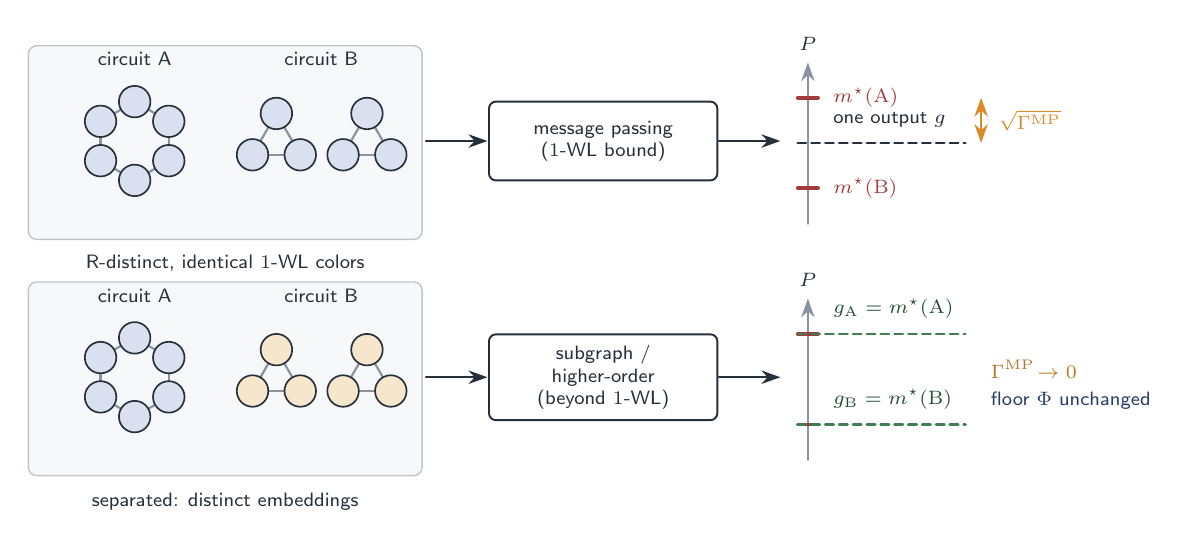
\begin{tikzpicture}[font=\sffamily, line cap=round, line join=round]

% ===================== ROW 1: message passing is stuck =====================
\draw[panel] (0.10,2.70) rectangle (5.10,5.16);
\begin{scope}[shift={(1.45,3.95)}]
  \foreach \i in {0,...,5}{\coordinate (A\i) at ({90+60*\i}:0.50);}
  \foreach \i in {0,...,5}{\pgfmathtruncatemacro{\j}{mod(\i+1,6)}
     \draw[edgegray,line width=0.8pt] (A\i)--(A\j);}
  \foreach \i in {0,...,5}{\node[gnode,minimum size=4mm,fill=floorlt] at (A\i) {};}
\end{scope}
\begin{scope}[shift={(3.25,3.95)}]
  \foreach \i in {0,1,2}{\coordinate (B\i) at ({90+120*\i}:0.35);}
  \foreach \i in {0,1,2}{\pgfmathtruncatemacro{\j}{mod(\i+1,3)}
     \draw[edgegray,line width=0.8pt] (B\i)--(B\j);}
  \foreach \i in {0,1,2}{\node[gnode,minimum size=4mm,fill=floorlt] at (B\i) {};}
\end{scope}
\begin{scope}[shift={(4.40,3.95)}]
  \foreach \i in {0,1,2}{\coordinate (C\i) at ({90+120*\i}:0.35);}
  \foreach \i in {0,1,2}{\pgfmathtruncatemacro{\j}{mod(\i+1,3)}
     \draw[edgegray,line width=0.8pt] (C\i)--(C\j);}
  \foreach \i in {0,1,2}{\node[gnode,minimum size=4mm,fill=floorlt] at (C\i) {};}
\end{scope}
\node[figsmall, anchor=south] at (1.45,4.78) {circuit A};
\node[figsmall, anchor=south] at (3.82,4.78) {circuit B};
\node[figsmall, anchor=north] at (2.60,2.62) {$\R$-distinct, identical $1$-WL colors};

\draw[->, line width=0.9pt, ink] (5.15,3.95) -- (5.93,3.95);
\node[chip, font=\sffamily\scriptsize, minimum width=2.9cm, minimum height=1.0cm]
  (mp) at (7.40,3.95) {message passing\\($1$-WL bound)};
\draw[->, line width=0.9pt, ink] (8.87,3.95) -- (9.65,3.95);

\begin{scope}[shift={(10.00,3.10)}]
  \draw[edgegray, ->, line width=0.8pt] (0,-0.20) -- (0,1.85);
  \node[ink, font=\sffamily\scriptsize, anchor=south] at (0,1.88) {$P$};
  \draw[simcol, line width=1.3pt] (-0.13,1.40) -- (0.13,1.40);
  \node[simcol, font=\sffamily\scriptsize, anchor=west] at (0.20,1.40) {$m^\star(\mathrm{A})$};
  \draw[simcol, line width=1.3pt] (-0.13,0.25) -- (0.13,0.25);
  \node[simcol, font=\sffamily\scriptsize, anchor=west] at (0.20,0.25) {$m^\star(\mathrm{B})$};
  \draw[ink, densely dashed, line width=1.0pt] (-0.13,0.825) -- (2.00,0.825);
  \node[ink, font=\sffamily\scriptsize, anchor=south west] at (0.20,0.90) {one output $g$};
  \draw[<->, gapcol, line width=0.9pt] (2.20,0.825) -- (2.20,1.40);
  \node[gapcol, font=\sffamily\scriptsize, anchor=west] at (2.30,1.11)
    {$\sqrt{\Gamma^{\mathrm{MP}}}$};
\end{scope}

% ===================== ROW 2: a finer encoder separates them =====================
\draw[panel] (0.10,-0.30) rectangle (5.10,2.16);
\begin{scope}[shift={(1.45,0.95)}]
  \foreach \i in {0,...,5}{\coordinate (D\i) at ({90+60*\i}:0.50);}
  \foreach \i in {0,...,5}{\pgfmathtruncatemacro{\j}{mod(\i+1,6)}
     \draw[edgegray,line width=0.8pt] (D\i)--(D\j);}
  \foreach \i in {0,...,5}{\node[gnode,minimum size=4mm,fill=floorlt] at (D\i) {};}
\end{scope}
\begin{scope}[shift={(3.25,0.95)}]
  \foreach \i in {0,1,2}{\coordinate (E\i) at ({90+120*\i}:0.35);}
  \foreach \i in {0,1,2}{\pgfmathtruncatemacro{\j}{mod(\i+1,3)}
     \draw[edgegray,line width=0.8pt] (E\i)--(E\j);}
  \foreach \i in {0,1,2}{\node[gnode,minimum size=4mm,fill=gaplt] at (E\i) {};}
\end{scope}
\begin{scope}[shift={(4.40,0.95)}]
  \foreach \i in {0,1,2}{\coordinate (F\i) at ({90+120*\i}:0.35);}
  \foreach \i in {0,1,2}{\pgfmathtruncatemacro{\j}{mod(\i+1,3)}
     \draw[edgegray,line width=0.8pt] (F\i)--(F\j);}
  \foreach \i in {0,1,2}{\node[gnode,minimum size=4mm,fill=gaplt] at (F\i) {};}
\end{scope}
\node[figsmall, anchor=south] at (1.45,1.78) {circuit A};
\node[figsmall, anchor=south] at (3.82,1.78) {circuit B};
\node[figsmall, anchor=north] at (2.60,-0.40) {separated: distinct embeddings};

\draw[->, line width=0.9pt, ink] (5.15,0.95) -- (5.93,0.95);
\node[chip, font=\sffamily\scriptsize, minimum width=2.9cm, minimum height=1.0cm]
  (bw) at (7.40,0.95) {subgraph /\\higher-order\\(beyond $1$-WL)};
\draw[->, line width=0.9pt, ink] (8.87,0.95) -- (9.65,0.95);

\begin{scope}[shift={(10.00,0.10)}]
  \draw[edgegray, ->, line width=0.8pt] (0,-0.20) -- (0,1.85);
  \node[ink, font=\sffamily\scriptsize, anchor=south] at (0,1.88) {$P$};
  \draw[simcol, line width=1.3pt] (-0.13,1.40) -- (0.13,1.40);
  \draw[simcol, line width=1.3pt] (-0.13,0.25) -- (0.13,0.25);
  \draw[okcol, densely dashed, line width=1.0pt] (-0.13,1.40) -- (2.00,1.40);
  \draw[okcol, densely dashed, line width=1.0pt] (-0.13,0.25) -- (2.00,0.25);
  \node[okcol!62!black, font=\sffamily\scriptsize, anchor=south west] at (0.20,1.47)
    {$g_{\mathrm{A}}=m^\star(\mathrm{A})$};
  \node[okcol!62!black, font=\sffamily\scriptsize, anchor=south west] at (0.20,0.32)
    {$g_{\mathrm{B}}=m^\star(\mathrm{B})$};
  \node[gapcol!85!black, font=\sffamily\scriptsize, anchor=west] at (2.20,0.95)
    {$\Gamma^{\mathrm{MP}}\!\to 0$};
  \node[floorcol, font=\sffamily\scriptsize, anchor=west] at (2.20,0.55)
    {floor $\Phi$ unchanged};
\end{scope}

\end{tikzpicture}%
}
\caption{\textbf{The message-passing gap, and what closes it.}
\panellab{Top:} circuits A (a six-cycle) and B (two disjoint triangles) are
non-isomorphic, yet under uniform initial colors $1$-WL assigns them identical colorings,
so \emph{every} message-passing GNN maps them to one embedding and one output $g$, forced
to the conditional mean of the property over the $1$-WL class. The residual spread is the
gap: when the two classes are equally likely, $\sqrt{\Gamma^{\mathrm{MP}}}$ is the distance
from $g$ to either class mean (\cref{thm:wlgap}).
\panellab{Bottom:} an encoder that separates the two classes, such as a subgraph or
higher-order GNN, drives $\Gamma^{\mathrm{MP}}$ to zero and recovers each class mean, while
the floor $\Phi$, the variance of the property \emph{within} a representation class, is
untouched (\cref{cor:mono}). Values are illustrative; the $1$-WL collision is exact.}
\label{fig:wlgap}
\end{figure}

\begin{corollary}[Expressiveness closes the gap, never the floor]
\label{cor:mono}
Consider any encoder class whose outputs are deterministic functions of $\R$ that are constant on the cells of a partition $\W'$ with $\W_\R\subseteq\W'\subseteq\sigma(\R)$, that is, any class at least as fine as $1$-WL and no finer than $\R$ itself. Higher-order and subgraph GNNs, flow attention, and deterministic positional features are of this form. For such a class the attainable gap is at least $\E[\Var(m^\star\mid\W')]$, with equality when the class is $L^2$-dense in the $\W'$-measurable functions. That quantity is non-increasing as $\W'$ refines and equals $0$ once $\W'$ separates the $\R$-classes, so that $m^\star$ is $\W'$-measurable. Throughout, $\Phi(\R,P)$ is unchanged: expressiveness is a lever on the gap and none on the floor.
\end{corollary}

\begin{proof}
Refining the conditioning $\sigma$-algebra cannot increase expected conditional variance (\cref{fact:ltv} with $\W'\subseteq\W''$ gives $\E[\Var(m^\star\mid\W'')]\le\E[\Var(m^\star\mid\W')]$). When $\W'$ separates $\R$-classes, $m^\star$ is $\W'$-measurable, so $\Var(m^\star\mid\W')=0$ almost surely. $\Phi(\R,P)=\E[\Var(P\mid\R)]$ depends only on $\R$ and $P$.
\end{proof}

\noindent\emph{Randomized encoders.} Random node features \citep{sato2021random} are not functions of $\R$, so they sit outside the ranking above. They do not escape the floor either: for a predictor $g(\R,U)$ with $U$ independent of $(P,\R)$, conditioning on $(\R,U)$ gives $\E[(P-g)^2]=\Phi(\R,P)+\E[(m^\star-g)^2]\ge\Phi(\R,P)$, so \cref{cor:indep} applies unchanged.

\paragraph{A ladder of representations.}
Because the floor moves only with $\R$, the scientific object is the floor's behavior along a ladder of the representations the field actually uses (\cref{tab:ladder}). The rungs are nested: each is a refinement of the previous ($\R_i$ is a deterministic function of $\R_{i+1}$).

\begin{proposition}[Floor monotonicity and the simulation limit]
\label{prop:ladder}
For nested rungs $\R_0\sqsubseteq\cdots\sqsubseteq\R_L$, the floors are non-increasing,
\[
\Phi(\R_0,P)\ge \Phi(\R_1,P)\ge\cdots\ge \Phi(\R_L,P).
\]
Let $\design$ denote the netlist a circuit graph encodes (its topology, sized devices, terminal roles, and orientation). Suppose the finest rung encodes that netlist injectively, so that $\sigma(\R_L)=\sigma(\design)$. Then
\begin{equation}
\Phi(\R_L,P)=\E\!\big[\Var(P\mid \design)\big],
\label{eq:simlimit}
\end{equation}
the error attributable to factors outside the netlist. In particular $\Phi(\R_L,P)>0$ if and only if $P$ is not almost surely a deterministic function of $\design$, that is, if and only if $P$ depends on quantities the netlist does not carry, such as layout parasitics, process corners, or device mismatch. A property is graph-underdetermined exactly in this case; then every rung has floor at least $\Phi(\R_L,P)$, so no GNN on any rung and at any expressiveness can predict $P$ with error below this residual. Closing it requires information the netlist omits, such as extracted parasitics or an explicit corner and mismatch specification, which is what a full simulation flow supplies downstream; a netlist-level solver is subject to the same limit. If instead $\R_L$ quantizes device values then $\sigma(\R_L)\subseteq\sigma(\design)$ and \cref{eq:simlimit} weakens to $\Phi(\R_L,P)\ge\E[\Var(P\mid\design)]$, which leaves the impossibility conclusion intact because the floor is then larger.
\end{proposition}

\begin{proof}
Monotonicity is \cref{fact:ltv} applied to the nested $\sigma$-algebras $\sigma(\R_0)\subseteq\cdots\subseteq\sigma(\R_L)$. Since $\sigma(\R_L)=\sigma(\design)$, $\Var(P\mid\R_L)=\Var(P\mid\design)$ almost surely, giving \cref{eq:simlimit}; and $\E[\Var(P\mid\design)]=0$ iff $\Var(P\mid\design)=0$ a.s., i.e.\ iff $P$ is a.s.\ a measurable function of $\design$.
\end{proof}

The empirical question is \emph{where}, per property, the floor falls to near zero. A property whose floor vanishes by a coarse rung is graph-determined there: the task reduces to closing $\Gamma$, which the encoder ladder does (\cref{thm:wlgap,cor:mono}). A property whose floor remains bounded away from zero at the finest rung is graph-underdetermined by \cref{prop:ladder}. On a benchmark whose labels are a deterministic function of the design, \cref{eq:simlimit} equals zero and the informative output is the per-property minimum sufficient rung; a persistent floor requires label variation from outside the design. The protocol determines which case holds for each property.

% ---------------- LADDER TABLE ----------------
\begin{table}[t]
\centering
\caption{\textbf{The representation ladder.} Each rung adds information used somewhere in the circuit-GNN literature. Shading depth on the rung marks increasing information content; floors are non-increasing down the ladder (\cref{prop:ladder}). The experiments locate, per property, the rung at which the floor reaches (or fails to reach) near zero.}
\label{tab:ladder}
\setlength{\tabcolsep}{7pt}
\renewcommand{\arraystretch}{1.32}
\resizebox{\linewidth}{!}{%
\begin{tabular}{>{\centering\arraybackslash}m{1.0cm} l l l}
\toprule
\rowcolor{headbg}
\thead{Rung} & \thead{Representation $\R_i$} & \thead{What it adds} & \thead{Used by} \\
\midrule
\cellcolor{floorcol!8}\textbf{$\R_0$}  & Bare topology  & connectivity only (no types, no values)        & structural baseline \\
\cellcolor{floorcol!17}\textbf{$\R_1$} & Typed topology & component-type labels                          & net-level GNN input \citep{mehradfar2025falcon} \\
\cellcolor{floorcol!26}\textbf{$\R_2$} & Sized graph    & quantized device values (untyped terminals)    & CktGNN-style \citep{dong2023cktgnn} \\
\cellcolor{floorcol!35}\textbf{$\R_3$} & Ported netlist & terminal identity (gate/drain/source, $+/-$)   & terminal-level \citep{asadi2025rfinformed,pan2025gnnaclp} \\
\cellcolor{floorcol!44}\textbf{$\R_4$} & Ported + flow  & orientation / Kirchhoff structure              & flow attention \citep{plettenberg2025flow} \\
\bottomrule
\end{tabular}}
\end{table}

% ===================================================================
\section{Estimating the Floor}
\label{sec:estimators}
% ===================================================================

The floor $\Phi(\R,P)=\E[\Var(P\mid\R)]$ is estimated from a finite sample of circuits with SPICE labels. We give two estimators with complementary assumptions; the analysis code implements both.

\paragraph{Partition estimator (exact collisions).}
Group circuits into $\R$-equivalence classes by a graph-isomorphism-with-features hash (color refinement to a fixed point, then canonical sort). For a class $k$ with $n_k\ge 2$ members and property values $\{P_{k,j}\}$, the within-class sample variance is $s_k^2$. The pooled estimator is
\begin{equation}
\widehat{\Phi} \;=\; \frac{\sum_{k:\,n_k\ge 2}(n_k-1)\,s_k^2}{\sum_{k:\,n_k\ge 2}(n_k-1)} .
\label{eq:partition}
\end{equation}
This is exact and assumption-light where collisions are plentiful ($\R_0,\R_1$, and $\R_2$ under quantization). Where collisions are sparse (fine features at $\R_3,\R_4$), it uses few classes and we report its coverage, the fraction of circuits lying in non-singleton classes, alongside every estimate. The next proposition states precisely what \cref{eq:partition} estimates, which is what makes coverage the right thing to report.

\begin{proposition}[What the partition estimator measures]
\label{prop:estimator}
Condition on the realized partition of the sample into $\R$-classes, and assume the property values within each class are independent draws from that class's conditional law (as holds when circuits are sampled independently). Then $\widehat{\Phi}$ of \cref{eq:partition} is unbiased for the coverage-restricted floor
\begin{equation}
\Phi_{\mathrm{cov}} \;\eqdef\; \frac{\sum_{k:\,n_k\ge 2}(n_k-1)\,\Var(P\mid \R=k)}{\sum_{k:\,n_k\ge 2}(n_k-1)},
\label{eq:phicov}
\end{equation}
the degrees-of-freedom-weighted average conditional variance over classes observed at least twice. Singleton classes contribute to $\Phi(\R,P)$ but not to $\widehat{\Phi}$, so $\Phi_{\mathrm{cov}}$ need not equal $\Phi(\R,P)$: classes observed at least twice are over-represented among high-probability classes, and the two coincide only when the conditional variance is unrelated to class probability. We therefore report the coverage $\rho$, the fraction of circuits in non-singleton classes, with every estimate, and read $\widehat{\Phi}$ as an estimate of $\Phi(\R,P)$ only where coverage is high. Under the null $P\perp\R$, $\E[\widehat{\Phi}]=\Var(P)$.
\end{proposition}

\begin{proof}
Within a class $k$ with $n_k\ge2$, the values are i.i.d.\ from the law of $P\mid\R=k$, so the sample variance $s_k^2$ is unbiased for $\Var(P\mid\R=k)$. By linearity, $\E[\widehat\Phi\mid\text{partition}]$ is the $(n_k-1)$-weighted average of these, namely \cref{eq:phicov}. Under $P\perp\R$ the within-class law equals the marginal, so $\Var(P\mid\R=k)=\Var(P)$ for every $k$ and the weighted average is $\Var(P)$.
\end{proof}

\paragraph{Neighborhood estimator (approximate collisions).}
Where exact collisions are rare, estimate $\Var(P\mid\R)$ locally: for each circuit, take its $\kappa$ nearest neighbors under a representation-space distance $\mathrm{dist}_\R$ (graph edit distance on the featured graph, or embedding distance from a fixed untrained encoder), and average the local variance. This trades an exactness assumption for a smoothness assumption ($m^\star$ Lipschitz in $\mathrm{dist}_\R$). Because $m^\star$ varies within a neighborhood, the local variance absorbs that variation as well, so the estimator is biased upward and can overstate the floor, which is the direction that would overstate impossibility. We report sensitivity to $\kappa$ and use it as a cross-check on the partition estimator rather than as the basis for a claim.

\paragraph{Confidence and honesty guards.}
All floor estimates carry bootstrap confidence intervals over circuits (class-resampled for the partition estimator). We additionally report (i) a permutation null in which $P$ is shuffled within the sample to confirm the estimator returns near total variance under no representation--property link, and (ii) the coverage of the partition estimator per rung. A high-floor claim is made only when the bootstrap interval lies entirely above the pre-registered tolerance, and a near-zero claim only when it lies entirely below it; the tolerance is fixed in the runbook before the runs.

\begin{algorithm}[t]
\caption{Per-property sufficiency floor along the representation ladder}
\label{alg:floor}
\begin{algorithmic}[1]
\Require circuits $\{c_i\}$ with SPICE labels $\{P_i\}$; ladder $\{\R_0,\dots,\R_L\}$
\For{each rung $\R_\ell$ and each property $P$}
  \State compute featured-graph canonical keys $\{\R_\ell(c_i)\}$ via color refinement
  \State partition into equivalence classes; compute $\widehat{\Phi}$ by \cref{eq:partition} and coverage
  \State bootstrap CI (class-resampled); permutation null; neighborhood cross-check
\EndFor
\State \Return floor curve $\ell\mapsto\widehat{\Phi}(\R_\ell,P)$ with CIs and coverage, per property
\end{algorithmic}
\end{algorithm}

% ===================================================================
\section{Experimental Design and Protocol}
\label{sec:experiments}
% ===================================================================

We describe the full protocol; all numbers below are placeholders (\RES{}) to be replaced by the runs. Results and Discussion are structured around the tables and figure the experiments will populate.

\paragraph{Data.}
The primary benchmark is FALCON \citep{mehradfar2025falcon}: roughly one million Cadence-simulated mm-wave circuits across five families (LNA, mixer, VCO, PA, VA) with native labels that include gain-type metrics, bandwidth, noise figure, and DC power. It is among the largest public analog-circuit datasets, and it labels noise figure and DC power directly, so metrics that would otherwise require re-simulation can be read from released data. The secondary benchmark is OCB \citep{dong2023cktgnn}, Ckt-Bench-101 (10k op-amps) and Ckt-Bench-301 (50k), a different circuit family (op-amps) with a different graph convention (DAGs), which tests whether the boundary generalizes across families and graph types. Primary properties on FALCON are DC gain (or power gain), bandwidth, noise figure, and DC power; on OCB, DC gain, bandwidth, phase margin, and figure of merit. We use each benchmark's released splits. (The exact FALCON field names, units, and redistribution license must be confirmed against the release before use; see the runbook.)

\paragraph{Ladder instantiation.}
$\R_0$--$\R_4$ per \cref{tab:ladder}, constructed from each benchmark's released netlists. On FALCON, the native net-level graph provides $\R_1$ and the terminal-annotated netlist provides $\R_3$, matching the net-level versus terminal-level contrast the RF SOTA studies \citep{asadi2025rfinformed}; $\R_2$ uses the released device values, and $\R_4$ adds edge orientation consistent with \citep{plettenberg2025flow}. On OCB, $\R_2$ uses CktGNN's native quantization and $\R_3$ adds terminal roles from the netlist. We verify, by direct count on the released data, the number and coverage of $\R$-equivalence classes at each rung before any floor is reported.

\paragraph{Encoder ladder (for the gap).}
To measure how close achievable error gets to the floor, we train at each representation rung a ladder of encoders spanning the current expressiveness frontier, so that a floor that survives the strongest model is a genuine limit rather than an artifact of a weak baseline. Three tiers: (i) \emph{$1$-WL message passing}, a GIN \citep{xu2019gin} (the reference class for \cref{thm:wlgap}), and the DAG encoders D-VAE and DAGNN on OCB \citep{zhang2019dvae,thost2021dagnn}; (ii) \emph{SOTA circuit predictors}, the strongest current models on these tasks, namely FALCON's net-level GNN \citep{mehradfar2025falcon}, the RF-informed terminal-level GENConv encoder \citep{asadi2025rfinformed}, the flow-attentional DAG encoder \citep{plettenberg2025flow}, and the self-supervised contrastive-pretrained encoder DICE \citep{lee2025dice}; and (iii) \emph{beyond-$1$-WL}, a subgraph GNN (ESAN) \citep{bevilacqua2022esan} and a graph transformer (GraphGPS with structural and positional encodings), which its authors argue is a universal function approximator on graphs \citep{rampasek2022graphgps} and which therefore serves as a stringent ceiling. Tier (iii) matters because \cref{thm:wlgap} bounds only the message-passing class. \Cref{cor:indep} covers the transformer case, since a graph transformer on $\R$ is still a function of $\R$; E3 and E7 test whether GraphGPS in fact plateaus at the floor for floor-limited properties.

\paragraph{Metrics and statistics.}
Per property we report: the estimated floor $\widehat{\Phi}$ with a bootstrap CI and coverage; the best test MSE/RMSE and Pearson $R$ over the encoder ladder; and the estimated gap (best achievable error minus floor). The gap carries its own uncertainty: we propagate the floor CI together with the model-error variance over ten seeds, so a ``floor-limited'' verdict requires the gap CI to include zero and a ``gap-limited'' verdict requires it to exclude zero. Trained models use ten seeds (mean $\pm$ std) with paired tests across encoders, on the normalized scale of \citep{dong2023cktgnn,plettenberg2025flow} for comparability. Because floors depend on the circuit distribution, we report them both aggregated and per FALCON family (LNA, mixer, VCO, PA, VA), since a property can be graph-determined in one family and not another. We also report the wall-clock cost of the floor computation, which is training-free and runs on CPU over the full million-circuit set, to substantiate that the headline analysis needs no GPU.

\paragraph{Protocol: positive control first.}
The instrument must pass a control before any headline claim: it must return a near-zero floor for a property that is known to be graph-determined. We choose DC power on FALCON and DC gain on OCB, both of which existing GNNs predict well \citep{mehradfar2025falcon,dong2023cktgnn,plettenberg2025flow}, and require a low floor by the sized-device rung with a 1-WL GIN already close to the floor. The per-metric errors that motivate this choice are to be read off the released tables of the cited work and recorded in the runbook before E1 is run. If the control does not come out easy, the pipeline is broken and no other result is trusted. We deliberately do \emph{not} use FALCON gain-type metrics as the control, because the RF SOTA reports them among the \emph{harder} metrics, which is itself part of what E2 investigates.

\torun{\textbf{E1 (positive control, run first).} Floor at $\R_2$ via \cref{alg:floor} for DC power on FALCON and DC gain on Ckt-Bench-101; train GIN/DAGNN/Flow-DAGNN at $\R_2$. \emph{Expected:} $\widehat{\Phi}(\R_2,\cdot)\!\approx\!\RES$ (near zero relative to total variance), best GNN RMSE $\!\approx\!\RES$ within CI of the floor. Supports the instrument's validity; if it fails, stop and debug. Reduces the risk that later ``high floor'' claims are optimization or pipeline artifacts.}

\torun{\textbf{E2 (floor curves, main result).} Compute $\widehat{\Phi}(\R_\ell,P)$ for $\ell=0..4$ on FALCON for $P\in\{$gain-type, bandwidth, noise figure, DC power$\}$ and on OCB for $P\in\{$gain, bandwidth, phase margin, FoM$\}$. The primary object is the \emph{shape} of each curve, hence the \emph{minimum representation rung} at which each property's floor reaches tolerance. \emph{Expected:} monotone-decreasing curves that separate by property, with easy metrics (DC power, and on OCB gain) resolving at a coarse rung and others resolving only at finer rungs. Whether any property's floor persists at $\R_4$ is the open empirical question, not an assumption: on a dataset whose labels are a deterministic function of the sized netlist, all floors may reach tolerance by $\R_4$, in which case the finding is the per-property minimum sufficient rung; a floor that persists at $\R_4$ requires label variation no graph rung captures (layout parasitics, process corners, or device mismatch), and we report which regime each property falls in rather than presupposing it. Produces \cref{fig:floorcurve} and \cref{tab:main}.}

\torun{\textbf{E3 (gap vs.\ floor).} At each rung, take the best GNN error across the encoder ladder and report gap $=$ error $-$ floor. \emph{Expected:} which term dominates is exactly what is unknown a priori and what the decomposition resolves; we expect at least one property that is gap-dominated at coarse rungs (total error falls as expressiveness rises, toward the floor) and at least one that is floor-dominated (total error plateaus above the floor no matter the encoder). This directly tests \cref{thm:wlgap,cor:mono}: expressiveness closes the gap, never the floor.}

\torun{\textbf{E4 (collision case studies).} Extract concrete $\R$-equivalent circuit pairs at $\R_3/\R_4$ with large property spread and explain the responsible physics (e.g., bias-dependent $g_m$, parasitic caps, matching). \emph{Expected:} a small gallery that attaches a physical mechanism to the floor, which also answers the objection that the floor is an artifact of the partition.}

\torun{\textbf{E5 (cross-benchmark consistency).} For the properties shared across both benchmarks (gain, bandwidth), compare the minimum sufficient rung and the floor-curve shape on FALCON versus OCB. \emph{Expected:} the qualitative per-property pattern agrees across two circuit families and two graph conventions, so the finding is a property of the representation--physics relationship and not of one dataset. Disagreement is reported as scope. Re-simulation via OCB's simulator remains available only for properties neither benchmark labels (e.g., PSRR); FALCON labels noise figure and DC power natively.}

\torun{\textbf{E6 (decomposition vs.\ the leaderboard, the justifying experiment).} Reproduce, within tolerance, the per-metric total errors reported by the SOTA circuit predictors (FALCON's net-level GNN and the RF-informed terminal-level model) on their released data, then decompose each into floor and gap via \cref{alg:floor} and the trained-error ceiling. \emph{Expected:} at least one metric whose competitive leaderboard error is dominated by the \emph{floor} (so the leaderboard-implied ``improve the architecture'' conclusion is misdirected), alongside a metric with a similar total error that is \emph{gap}-dominated (where a better encoder does help). This is the paper's operative claim: the total error the field reports conflates two limits with opposite remedies, and the decomposition changes the recommended action. Produces \cref{tab:sota}.}

\torun{\textbf{E7 (oracle validation of the simulation limit).} On a subset, inject a controlled amount of non-netlist variation into the labels by re-simulating with a known spread of device mismatch or process corners (or calibrated Monte-Carlo), sweeping the injected variance. \emph{Expected:} the estimated floor at $\R_4$ tracks the injected variance across the sweep, validating \cref{eq:simlimit} (the floor equals the variance from factors outside the netlist), and no encoder in the ladder, including the GraphGPS transformer, drives error below it. This validates \cref{prop:ladder} end to end and exhibits the mechanism behind a persistent floor rather than inferring it; without an injection run, the persistent-floor question is reported as open.}

\torun{\textbf{E8 (estimator robustness, instrument validation).} (a) Quantization sensitivity: recompute the $\R_2$ floor across device-value bin widths and report stability. (b) Estimator agreement: at rungs with adequate coverage, check that the partition and neighborhood estimators (\cref{sec:estimators}) agree within CIs. (c) Independent cross-estimator: compare the conditional-variance floor to an information-theoretic irreducible-error estimate (a $k$NN mutual-information estimator, in the spirit of \citep{dimensionless2025irreducible}) on the same partition. (d) Coverage convergence: show $\widehat{\Phi}$ stabilizes as the sample grows and coverage rises. (e) Label precision: verify the floor is not an artifact of finite SPICE label precision by re-estimating under added label quantization. \emph{Expected:} the floor estimate is stable across (a)--(e), with disagreements reported. Establishes that the floor originates in the data and the representation.}

% ---------------- MAIN RESULTS TABLE (placeholders) ----------------
\begin{table}[t]
\centering
\caption{\textbf{Main results (placeholders).} Per property and rung: the training-free sufficiency floor $\widehat{\Phi}$ with coverage, the best error over the full encoder ladder, and the gap. Filled by E2--E3. Read-out: a near-zero floor at some rung means a GNN can replace the simulator for that property (\emph{graph-determined}); a floor that stays high at $\R_4$ means it cannot (\emph{simulation-required}). Verdicts are placeholders and will be colored by the measured floor once E2--E3 run.}
\label{tab:main}
\setlength{\tabcolsep}{6pt}
\renewcommand{\arraystretch}{1.22}
\resizebox{\linewidth}{!}{%
\begin{tabular}{l c c c c c l}
\toprule
\rowcolor{headbg}
 & & \multicolumn{2}{c}{\cellcolor{headbg}\thead{Sufficiency floor\\(training-free)}} & \multicolumn{2}{c}{\cellcolor{headbg}\thead{Best achievable\\(encoder ladder)}} & \\
\rowcolor{headbg}
\multirow{-2}{*}{\thead{Property}} & \multirow{-2}{*}{\thead{Rung}} & \thead{$\widehat{\Phi}$} & \thead{coverage} & \thead{RMSE} & \thead{gap} & \multirow{-2}{*}{\thead{Verdict}} \\
\cmidrule(lr){3-4}\cmidrule(lr){5-6}
\multicolumn{7}{l}{\cellcolor{floorcol!7}\textit{FALCON}: mm-wave; noise figure and DC power are native labels}\\
Gain          & $\R_2$ & \RES & \RES & \RES & \RES & \PH{regime} \\
Bandwidth     & $\R_2$ & \RES & \RES & \RES & \RES & \PH{regime} \\
Bandwidth     & $\R_4$ & \RES & \RES & \RES & \RES & \PH{regime} \\
DC power      & $\R_3$ & \RES & \RES & \RES & \RES & \PH{regime} \\
Noise figure  & $\R_2$ & \RES & \RES & \RES & \RES & \PH{regime} \\
Noise figure  & $\R_4$ & \RES & \RES & \RES & \RES & \PH{regime} \\
\addlinespace[1pt]
\multicolumn{7}{l}{\cellcolor{floorcol!7}\textit{OCB}: op-amps (directed acyclic graphs)}\\
Phase margin  & $\R_4$ & \RES & \RES & \RES & \RES & \PH{regime} \\
FoM           & $\R_4$ & \RES & \RES & \RES & \RES & \PH{regime} \\
\bottomrule
\end{tabular}}
\vspace{2pt}
{\footnotesize The gap carries a propagated CI; a floor-limited verdict requires the gap CI to include zero, a gap-limited verdict requires it to exclude zero. All $\widehat{\Phi}$ and errors are on the normalized scale of \citep{dong2023cktgnn,plettenberg2025flow}.}
\end{table}

% ---------------- SOTA DECOMPOSITION TABLE (E6, placeholders) ----------------
\begin{table}[t]
\centering
\caption{\textbf{Decomposing the leaderboard (placeholders, E6).} For each SOTA circuit predictor and metric, the reported total error (reproduced within tolerance) split by \cref{alg:floor} into the encoder-independent floor and the closable gap. The operative point: two metrics with similar total error can differ in whether the residual is a \emph{floor} (invest in richer inputs or simulation) or a \emph{gap} (invest in a better encoder), which the leaderboard number alone cannot tell apart. Verdicts are placeholders, colored once measured.}
\label{tab:sota}
\setlength{\tabcolsep}{6pt}
\renewcommand{\arraystretch}{1.22}
\resizebox{\linewidth}{!}{%
\begin{tabular}{l l c c c l}
\toprule
\rowcolor{headbg}
 & & \multicolumn{3}{c}{\cellcolor{headbg}\thead{Error decomposition\ \ ($\text{total}^2=\Phi+\Gamma$)}} & \\
\rowcolor{headbg}
\multirow{-2}{*}{\thead{SOTA model}} & \multirow{-2}{*}{\thead{Metric}} & \thead{total} & \thead{floor $\widehat{\Phi}$} & \thead{gap} & \multirow{-2}{*}{\thead{Verdict}} \\
\cmidrule(lr){3-5}
\multirow{2}{*}{\makecell[tl]{FALCON\\{\footnotesize net-level \citep{mehradfar2025falcon}}}}
                       & DC power     & \RES & \RES & \RES & \PH{regime} \\
                       & gain-type    & \RES & \RES & \RES & \PH{regime} \\
\addlinespace[1pt]
\multirow{2}{*}{\makecell[tl]{RF-informed\\{\footnotesize terminal \citep{asadi2025rfinformed}}}}
                       & noise figure & \RES & \RES & \RES & \PH{regime} \\
                       & efficiency   & \RES & \RES & \RES & \PH{regime} \\
\bottomrule
\end{tabular}}
\vspace{2pt}
{\footnotesize ``total'' reproduces each source's released error within tolerance before decomposition; the verdict follows from whether the gap CI includes zero (floor-limited) or excludes it (gap-limited). Even the GraphGPS transformer cannot drive error below $\widehat{\Phi}$ (\cref{cor:indep}).}
\end{table}

% ---------------- FLOOR CURVE FIGURE (schematic, no data) ----------------
\begin{figure}[t]
\centering
\resizebox{\linewidth}{!}{%
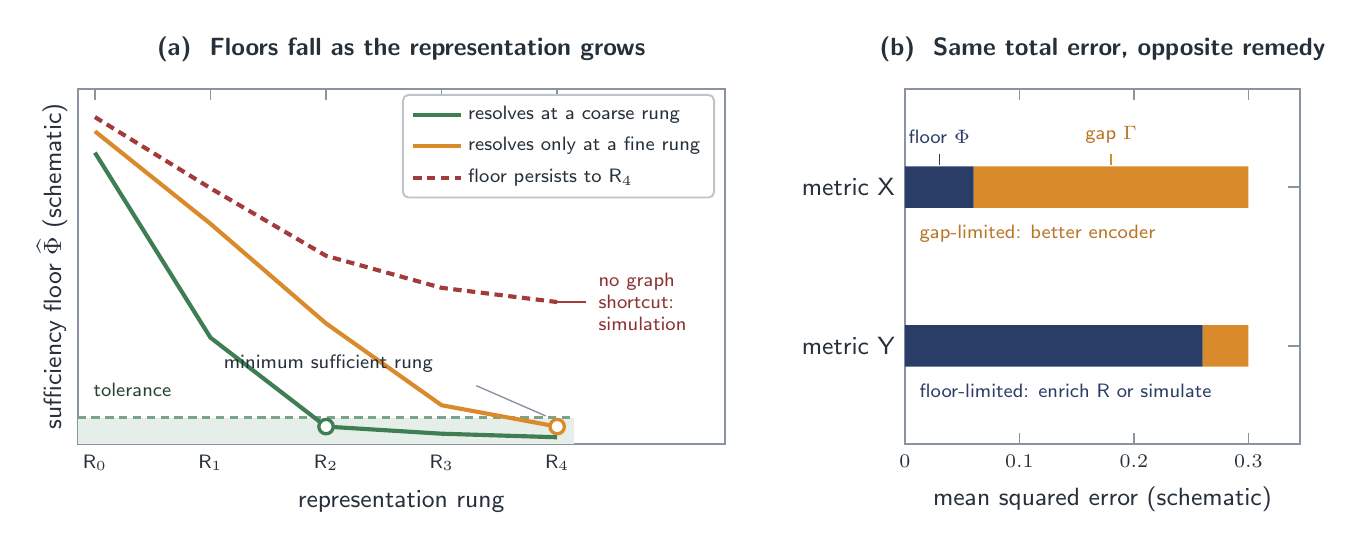
\begin{tikzpicture}
\begin{axis}[
  name=plotA,
  width=9.8cm, height=6.1cm,
  title={\textbf{(a)}\ \ Floors fall as the representation grows},
  xlabel={representation rung},
  ylabel={sufficiency floor $\widehat{\Phi}$ (schematic)},
  xtick={0,1,2,3,4},
  xticklabels={$\R_0$,$\R_1$,$\R_2$,$\R_3$,$\R_4$},
  ytick=\empty, ymin=0, ymax=1.0, xmin=-0.15, xmax=5.45,
  axis line style={draw=edgegray, line width=0.7pt},
  clip=false,
  legend style={at={(0.985,0.985)}, anchor=north east, legend cell align=left, row sep=1pt},
]
\fill[okcol!13] (axis cs:-0.15,0) rectangle (axis cs:4.15,0.075);
\draw[okcol!70, densely dashed, line width=0.9pt]
  (axis cs:-0.15,0.075) -- (axis cs:4.15,0.075);
\node[okcol!55!black, font=\sffamily\scriptsize, anchor=south west] at (axis cs:-0.10,0.105)
  {tolerance};
\addplot[line width=1.5pt, okcol] coordinates {(0,0.82)(1,0.30)(2,0.05)(3,0.03)(4,0.02)};
\addlegendentry{resolves at a coarse rung}
\addplot[line width=1.5pt, gapcol] coordinates {(0,0.88)(1,0.62)(2,0.34)(3,0.11)(4,0.05)};
\addlegendentry{resolves only at a fine rung}
\addplot[line width=1.5pt, simcol, densely dashed]
  coordinates {(0,0.92)(1,0.72)(2,0.53)(3,0.44)(4,0.40)};
\addlegendentry{floor persists to $\R_4$}
\draw[okcol,  fill=white, line width=1.2pt] (axis cs:2,0.05) circle (2.6pt);
\draw[gapcol, fill=white, line width=1.2pt] (axis cs:4,0.05) circle (2.6pt);
\node[ink, font=\sffamily\scriptsize, anchor=south] at (axis cs:2.02,0.175)
  {minimum sufficient rung};
\draw[edgegray, line width=0.5pt] (axis cs:3.30,0.165) -- (axis cs:3.90,0.080);
\draw[simcol, line width=0.6pt] (axis cs:4,0.40) -- (axis cs:4.25,0.40);
\node[simcol!85!black, font=\sffamily\scriptsize, align=left, anchor=west]
  at (axis cs:4.27,0.40) {no graph\\shortcut:\\simulation};
\end{axis}

\begin{axis}[
  name=plotB,
  at={(plotA.right of south east)}, anchor=left of south west, xshift=0.85cm,
  width=6.6cm, height=6.1cm,
  title={\textbf{(b)}\ \ Same total error, opposite remedy},
  xbar stacked, bar width=15pt,
  xmin=0, xmax=0.345,
  xtick={0,0.1,0.2,0.3},
  xlabel={mean squared error (schematic)},
  symbolic y coords={metric Y, metric X},
  ytick=data,
  yticklabel style={font=\sffamily\small},
  enlarge y limits=0.62,
  axis line style={draw=edgegray, line width=0.7pt},
  clip=false,
]
\addplot[fill=floorcol, draw=none] coordinates {(0.06,metric X) (0.26,metric Y)};
\addplot[fill=gapcol,   draw=none] coordinates {(0.24,metric X) (0.04,metric Y)};
% segment labels sit above the top bar so no fill can occlude them
\draw[floorcol, line width=0.5pt]
  ([yshift=8pt]axis cs:0.030,metric X) -- ([yshift=12pt]axis cs:0.030,metric X);
\draw[gapcol, line width=0.5pt]
  ([yshift=8pt]axis cs:0.180,metric X) -- ([yshift=12pt]axis cs:0.180,metric X);
\node[floorcol, font=\sffamily\scriptsize, anchor=south]
  at ([yshift=12pt]axis cs:0.030,metric X) {floor $\Phi$};
\node[gapcol!85!black, font=\sffamily\scriptsize, anchor=south]
  at ([yshift=12pt]axis cs:0.180,metric X) {gap $\Gamma$};
\node[gapcol!85!black, font=\sffamily\scriptsize, anchor=north west, yshift=-10pt]
  at (axis cs:0.004,metric X) {gap-limited: better encoder};
\node[floorcol, font=\sffamily\scriptsize, anchor=north west, yshift=-10pt]
  at (axis cs:0.004,metric Y) {floor-limited: enrich $\R$ or simulate};
\end{axis}
\end{tikzpicture}%
}
\caption{\textbf{Expected floor curves and the read-out (schematic; not measured).}
\panellab{(a)}~Floors are non-increasing along the ladder (\cref{prop:ladder}); the object
of interest is the rung at which each floor first drops below tolerance (open circles),
its minimum sufficient representation. A property may resolve at a coarse rung (green),
resolve only at a fine rung (amber), or retain a floor at $\R_4$ (red), where no GNN
offers a shortcut over simulation.
\panellab{(b)}~Why the split is worth measuring: two metrics with the \emph{same} total
error can decompose in opposite ways. The gap-limited metric rewards a better encoder;
the floor-limited metric does not, and calls instead for a richer representation or for
simulation. A leaderboard number alone cannot tell the two apart, which is what E6
measures. Both panels are schematic; the vertical axis in (a) and the bar lengths in (b)
carry no measured values.}
\label{fig:floorcurve}
\end{figure}

\paragraph{Results (to be written).}
We will report the floor curves (\cref{fig:floorcurve}), the per-property table (\cref{tab:main}), the case studies (E4), and the cross-benchmark consistency check (E5), then state, per property, the minimum sufficient rung, and whether any property's floor persists at $\R_4$ (where a GNN offers no shortcut over simulation). We will reconcile every abstract and contribution claim with these numbers, and soften the framing if the split is less sharp than hypothesized.

% ===================================================================
\section{Discussion}
% ===================================================================

\paragraph{What the boundary tells practitioners.}
The robust deliverable is a per-property \emph{minimum sufficient representation}: the coarsest graph rung at which a property's floor reaches tolerance. Below that rung, no architecture on that representation can succeed, and the return is in a richer input; at or above it, the residual is a gap and the encoder ladder is the right investment. The decomposition turns that judgment into a measurement, and it identifies a specific failure mode: improving a GNN's prediction of a property that is already gap-closed at the representation in use, where the visible ``improvement'' is noise around a floor. When a property's floor persists even at the richest practical representation, a GNN offers no shortcut over simulation for it; whether that occurs is one of the empirical questions the protocol settles.

\paragraph{Limitations.}
(i) Floors are defined against a distribution; ours are FALCON's five mm-wave families and OCB's op-amp space, and the boundary may shift for other families. The cross-benchmark check (E5) tests generality across two families and two graph conventions, but we report the outcome as a statement about these two settings. (ii) A persistent floor at the richest rung requires the labels to vary with factors no graph rung captures, such as layout parasitics, process corners, or device mismatch. On a dataset whose labels are a deterministic function of the sized netlist, floors may reach tolerance by $\R_4$, and the finding is then the per-property minimum sufficient rung. Which regime holds is settled by E2 and E7. (iii) The neighborhood estimator assumes smoothness of $m^\star$ in representation space; we use it only as a cross-check and report $\kappa$-sensitivity. (iv) Where exact collisions are sparse at fine rungs, the partition estimator has limited coverage; we disclose coverage and lean on E4 case studies for mechanism. (v) The theory is a specialization of classical results; its value is the split, instrument, and map, not new probability. The proof is elementary and stated in full, but we still recommend independent human verification of all formal claims.

\paragraph{Ethics and reproducibility.}
The study uses public benchmarks (FALCON and OCB) and released simulators; no human data. All floor computations are training-free and deterministic given the data; trained-model results use fixed seeds. We will release code for the estimators, the ladder construction, and the training harness, and will confirm each benchmark's redistribution license before releasing any derived artifact.

% ===================================================================
\section{Conclusion}
% ===================================================================

The question of where GNNs can replace circuit simulation has been pursued mainly by building better models, both more expressive encoders and richer graph abstractions. We separated two limits that this conflates: an encoder-independent representation-sufficiency floor and a closable expressiveness gap, proved they add, and specified a ladder-based instrument for measuring, per property, the minimum representation at which the floor reaches tolerance on two public benchmarks. This turns the field's recurring observation that accuracy is representation-bound and property-specific into a measured quantity, and gives concrete guidance on when architecture versus richer inputs is the right lever. The empirical map awaits the runs specified here. The claims are stated so that those runs can falsify them, and every number in this draft is a visible placeholder.

% ===================================================================
\bibliographystyle{plainnat}
\bibliography{simboundary}
% ===================================================================

\appendix
\section{Classical facts and the proof of \cref{thm:decomp}}
\label{app:proof}

The main-text results build on two standard facts, collected here so the novel proofs in \cref{sec:theory} are self-contained. Throughout, $P$ has $\E[P^2]<\infty$.

\begin{fact}[$L^2$ projection]
\label{fact:proj}
For a $\sigma$-algebra $\mathcal{A}$, the conditional expectation $\E[P\mid\mathcal{A}]$ is the $L^2$-orthogonal projection of $P$ onto $\mathcal{A}$-measurable functions: $\E[(P-\E[P\mid\mathcal{A}])\,u]=0$ for every $\mathcal{A}$-measurable $u$ with $\E[u^2]<\infty$, and $\E[P\mid\mathcal{A}]$ minimizes $\E[(P-u)^2]$ over such $u$, with minimum $\E[\Var(P\mid\mathcal{A})]$.
\end{fact}

\begin{fact}[Nested law of total variance]
\label{fact:ltv}
For $\sigma$-algebras $\mathcal{A}\subseteq\mathcal{B}$,
\[
\E\!\big[\Var(P\mid\mathcal{A})\big] \;=\; \E\!\big[\Var(P\mid\mathcal{B})\big] \;+\; \E\!\big[\Var(\E[P\mid\mathcal{B}]\mid\mathcal{A})\big].
\]
In particular $\E[\Var(P\mid\mathcal{A})]\ge\E[\Var(P\mid\mathcal{B})]$: conditioning on a refinement never increases expected conditional variance.
\end{fact}

Both are classical \citep{hastie2009esl,devroye1996probabilistic,cover2006information}; \cref{fact:ltv} follows by applying the tower property to $\Var(P\mid\mathcal{A})=\E[P^2\mid\mathcal{A}]-\E[P\mid\mathcal{A}]^2$ and using $\E[P\mid\mathcal{A}]=\E[\E[P\mid\mathcal{B}]\mid\mathcal{A}]$.

\medskip
\noindent\textit{Proof of \cref{thm:decomp}.} Let $m^\star=\E[P\mid\R]$ and let $g=h\circ\R$ be any $\R$-measurable predictor with $\E[g^2]<\infty$. Write $P-g=(P-m^\star)+(m^\star-g)$. Since $m^\star-g$ is $\R$-measurable, \cref{fact:proj} gives $\E[(P-m^\star)(m^\star-g)]=0$, so
\[
\E[(P-g)^2] = \E[(P-m^\star)^2] + \E[(m^\star-g)^2].
\]
By \cref{fact:proj}, $\E[(P-m^\star)^2]=\E[\Var(P\mid\R)]=\Phi(\R,P)$, which is \cref{eq:pyth}. Taking the infimum over $g\in\Gcal_\R$ and noting $\Phi(\R,P)$ does not depend on $g$ yields \cref{eq:infdecomp} with $\Gamma(\Gcal_\R,P)=\inf_{g\in\Gcal_\R}\E[(m^\star-g)^2]\ge0$. \hfill$\square$

\section{Reproducibility and pre-registration}
\label{app:repro}
Before running, the authors fix: the tolerance defining ``near zero'' (as a fraction of each property's total variance); the bootstrap resample count and seed; the neighborhood size $\kappa$ and distance $\mathrm{dist}_\R$; and the encoder-ladder hyperparameter budget. The partition estimator, coverage reporting, permutation null, and bootstrap are specified in \cref{alg:floor} and the released code. Trained-model results use ten seeds with reported variance. The venue reproducibility checklist will be completed at submission; formal claims are to be independently verified by the human authors, who take responsibility for all content.

\end{document}
